%input macros (i.e. write your own macros file called MacroFile1.tex)
%\newcommand{\PdfPsText}[2]{
  \ifpdf
     #1
  \else
     #2
  \fi
}

\newcommand{\IncludeGraphicsH}[3]{
  \PdfPsText{\includegraphics[height=#2]{#1}}{\includegraphics[bb = #3, height=#2]{#1}}
}

\newcommand{\IncludeGraphicsW}[3]{
  \PdfPsText{\includegraphics[width=#2]{#1}}{\includegraphics[bb = #3, width=#2]{#1}}
}

\newcommand{\InsertFig}[3]{
  \begin{figure}[!htbp]
    \begin{center}
      \leavevmode
      #1
      \caption{#2}
      \label{#3}
    \end{center}
  \end{figure}
}


%%% Local Variables: 
%%% mode: latex
%%% TeX-master: "~/Documents/LaTeX/CUEDThesisPSnPDF/thesis"
%%% End: 


 \documentclass[oneside,12pt]{Classes/CUEDthesisPSnPDF}

\title{Sign Align -- A System to Track and Translate Sign Language}
\author{Daniel Nichol}
\collegeordept{Department of Computer Science}
\university{University of Oxford}
\crest{}


\degree{Master of Mathematics and Computer Science}
\degreedate{}

% turn of those nasty overfull and underfull hboxes
\hbadness=10000
\hfuzz=50pt

% Put all the style files you want in the directory StyleFiles and usepackage like this:
\usepackage{StyleFiles/watermark}
\usepackage{amsmath,amsfonts,amsthm}
\usepackage{bm}

% Comment out the next line to get single spacing
\onehalfspacing

\begin{document}

%\language{english}

% A page with the abstract on including title and author etc may be
% required to be handed in separately. If this is not so, then comment
% the below 3 lines (between '\begin{abstractseparte}' and 
% 'end{abstractseparate}'), normally like a declaration ... needs some more
% work, mind as environment abstracts creates a new page!
% \begin{abstractseparate}
%   
% Thesis Abstract -----------------------------------------------------


%\begin{abstractslong}    %uncommenting this line, gives a different abstract heading
\begin{abstracts}        %this creates the heading for the abstract page

This is where you write your abstract ...


\end{abstracts}
%\end{abstractlongs}


% ----------------------------------------------------------------------


%%% Local Variables: 
%%% mode: latex
%%% TeX-master: "../thesis"
%%% End: 

% \end{abstractseparate}

\maketitle

%set the number of sectioning levels that get number and appear in the contents
\setcounter{secnumdepth}{3}
\setcounter{tocdepth}{3}

\frontmatter % book mode only
\pagenumbering{roman}
% Thesis Dedictation ---------------------------------------------------

\begin{dedication} %this creates the heading for the dedication page


\end{dedication}

% ----------------------------------------------------------------------

%%% Local Variables: 
%%% mode: latex
%%% TeX-master: "../thesis"
%%% End: 

% Thesis Acknowledgements ------------------------------------------------


%\begin{acknowledgementslong} %uncommenting this line, gives a different acknowledgements heading
\begin{acknowledgements}      %this creates the heading for the acknowlegments

\end{acknowledgements}
%\end{acknowledgmentslong}

% ------------------------------------------------------------------------

%%% Local Variables: 
%%% mode: latex
%%% TeX-master: "../thesis"
%%% End: 


% Thesis Abstract -----------------------------------------------------


%\begin{abstractslong}    %uncommenting this line, gives a different abstract heading
\begin{abstracts}        %this creates the heading for the abstract page

This is where you write your abstract ...


\end{abstracts}
%\end{abstractlongs}


% ----------------------------------------------------------------------


%%% Local Variables: 
%%% mode: latex
%%% TeX-master: "../thesis"
%%% End: 


\tableofcontents
\listoffigures
\printnomenclature  %% Print the nomenclature
\addcontentsline{toc}{chapter}{Nomenclature}

\mainmatter % book mode only
%%% Thesis Introduction --------------------------------------------------
\chapter{Introduction}
\ifpdf
    \graphicspath{{Introduction/IntroductionFigs/PNG/}{Introduction/IntroductionFigs/PDF/}{Introduction/IntroductionFigs/}}
\else
    \graphicspath{{Introduction/IntroductionFigs/EPS/}{Introduction/IntroductionFigs/}}
\fi

British Sign Language is the preferred first language of over 125,000 in the United Kingdom, in addition to an estimated 20,000 children and thousands of hearing friends, relatives and interpreters. There are many more people worldwide communicating in an estimated 200 different signed languages, with a huge variation in grammar and pronounciation. As such, a system which can recognise signed languages and convert them into text in real time would be a valuable tool for many people. 

The aim of this project is to implement a system to recognise gestures of a signed language from a continuous data stream provided from the Microsoft Kinect camera. The problem of continuous gesture recognition has been studied for over 20 years and has seen solutions which often involve specific gloves or expensive hardware and which have been particularly sensitive to lighting conditions and camera placement. Using the Kinect sensor, which is available to purchase off the shelf and is designed to be used without gloves and in a range of conditions, we aim to build a robust sign recognition system which does not suffer from these limitations.

\section{Sign Language}
Signed languages natural languages which have evolved independently of the spoken languages of the areas in which they are used and often independently of one another. For example, British Sign Language (BSL) is not simply oral English transcribed but rather a distinct language with its own sentence structure which differs significantly from English. Further despite the regions sharing a common language American Sign Language (ASL) is a seperate language from BSL.

Despite the large variation between regional sign languages the means of communication remain the same across most signed languages. The main component of the sign is the movement of the body and each sign is determined by the movement and location of the hands and arms as well as the hand shape and palm direction. In addition to the manual component of the signs the signer will often use posture, facial expressions, mouth shape or eye movements to convey meaning.

The non-manual components of sign language will be ignored for the purposes of this project. It should be noted that eye tracking and facial expression are essentially independent problems from that of gesture recognition and hence if solutions to the facial expression problem exist they may be combined with the work of this project to produce a more substantial sign recognition system.

We can further break the manual part of a sign in to two components. The first is the movement of the hand, arms and body over time and the second is the orientation of the hand throughout this movement. This is a sensible distinction to make as it helps reduce the number of distinct signs to differentiate between. As the same hand shape might be used with two different arm movements to produce different words, we can reduce the number of distinct gestures we wish to detect by detecting hand movement gestures and hand shapes and then combining the two to identify a sign.

In the next section we will see there is a limitation in our choice of hardware that makes hand shape detection a problem which is outside the scope of this project. However the above observation shows that the work in this project to detect arm and body gestures can be combined with future work to produce a system which will detect a signed language. Furthermore, a major task of this project is to implement a library of Hidden Markov Model sequence classifiers to detect gestures and this library can be used to detect hand shape gestures just as we use it here to detect body gestures. 

\section{Hardware}
The Kinect is a motion sensing camera designed by Microsoft and released in November 2010. The Kinect combines an RGB camera and an infrared depth sensor to detect objects in 3D space. The raw images of these sensors are combined using proprietary software to detect a human body as a skeleton, in particular the Kinect is capable of detecting the positions of the hands, elbows, shoulders and head as a point in 3D space.

Microsoft released the Kinect software development kit (SDK) for public use on January 16, 2011. This SDK allows developers build applications which interact with the proprietary skeleton tracking software using C\#, C++ or Visual Basic. In this project we will use this SDK to build the gesture recognition framework.

The Kinect camera was originially designed with the ability to detect hand and finger positions. In fact the original patent claims the device would be able to detect American Sign Language ~\cite{LATTA:2010:biblatex}. However this functionality was removed from the original release of the Kinect sensor. The SDK was updated to recognise open and closed hands on March 18th, 2013~\cite{Microsoft:2013:Online} and it is believed that the next iteration of the Kinect hardware will be able to fully detect hand gestures.

Third party hand gesture recognition frameworks do exist, however the most successful of these do not make use of the Kinect SDK and so do not make use of its features at all~\cite{Forth:2013:Online}. We aim to build a framework that will be easily extended when the capabilities of the Kinect are improved and for this reason we choose to only use the tools provided within the Kinect SDK.
\section{Outline}

%%% ----------------------------------------------------------------------


%%% Local Variables: 
%%% mode: latex
%%% TeX-master: "../thesis"
%%% End: 

% \pagebreak[4]
% \hspace*{1cm}
% \pagebreak[4]
% \hspace*{1cm}
% \pagebreak[4]

\chapter{Background and Model Selection}
\ifpdf
    \graphicspath{{Chapter1/Chapter1Figs/PNG/}{Chapter1/Chapter1Figs/PDF/}{Chapter1/Chapter1Figs/}}
\else
    \graphicspath{{Chapter1/Chapter1Figs/EPS/}{Chapter1/Chapter1Figs/}}
\fi

\section{Model Selection}

\section{Hidden Markov Models}
A \emph{hidden Markov Model} (HMM) is (following the definitions in ~\cite{rabiner1989tutorial}) a doubly stochastic process which consists of an underlying discrete Markov chain with state set $S = \{S_1, \dots, S_n \}$ and stochastic matrix $A=[a_{i,j}]_{N\times N}$ where 
\begin{equation*}
a_{i,j} = \mathbb{P}(q_{t+1} = S_i | q_t = S_j) \text{  for each  } 1 \leq i,j \leq N
\end{equation*}
which is hidden from an observer in the respect that one cannot directly observe the current state of the Markov chain. Instead we have a collection of $M$ observable symbols, say $V = \{ v_1, \dots, v_M\}$, which may be observed with probability dependent on the state underlying Markov chain (Figure:  ~\ref{fig:hmmex}). 

We encode these so-called \emph{emission probabilities} in a matrix $B = [b_j(k)]_{N\times M}$ where
\begin{equation*}
b_j(k) = \mathbb{P}[v_k \text{ occurs at time }t | q_t = S_j] 
\end{equation*}
Now if we take an initial state distribution $\bm{\pi} = [\pi_1, \dots, \pi_N]$ for our Markov chain with
\begin{equation*}
\pi_i= \mathbb{P}[q_1 = S_i]
\end{equation*}
Then the HMM generates a sequence of observations
\begin{equation*}
\bm{O} = O_1, O_2, \ldots , O_T
\end{equation*}
by the following process:
\begin{enumerate}
\item Choose an initial state $q_1 = S_i$ stochastically from the initial state distribution $\bm{\pi}$
\item For $t=1$ to $T$
\begin{enumerate}
\item[i.] Choose $O_t = v_k$ according to the distribution $b_i(k)$ of the current state $S_i$
\item[ii.] Stochastically transition to a new state $S_j$ from $S_i$ according to $A$ 
\end{enumerate}
\end{enumerate}

\begin{figure}[]
  \centering
    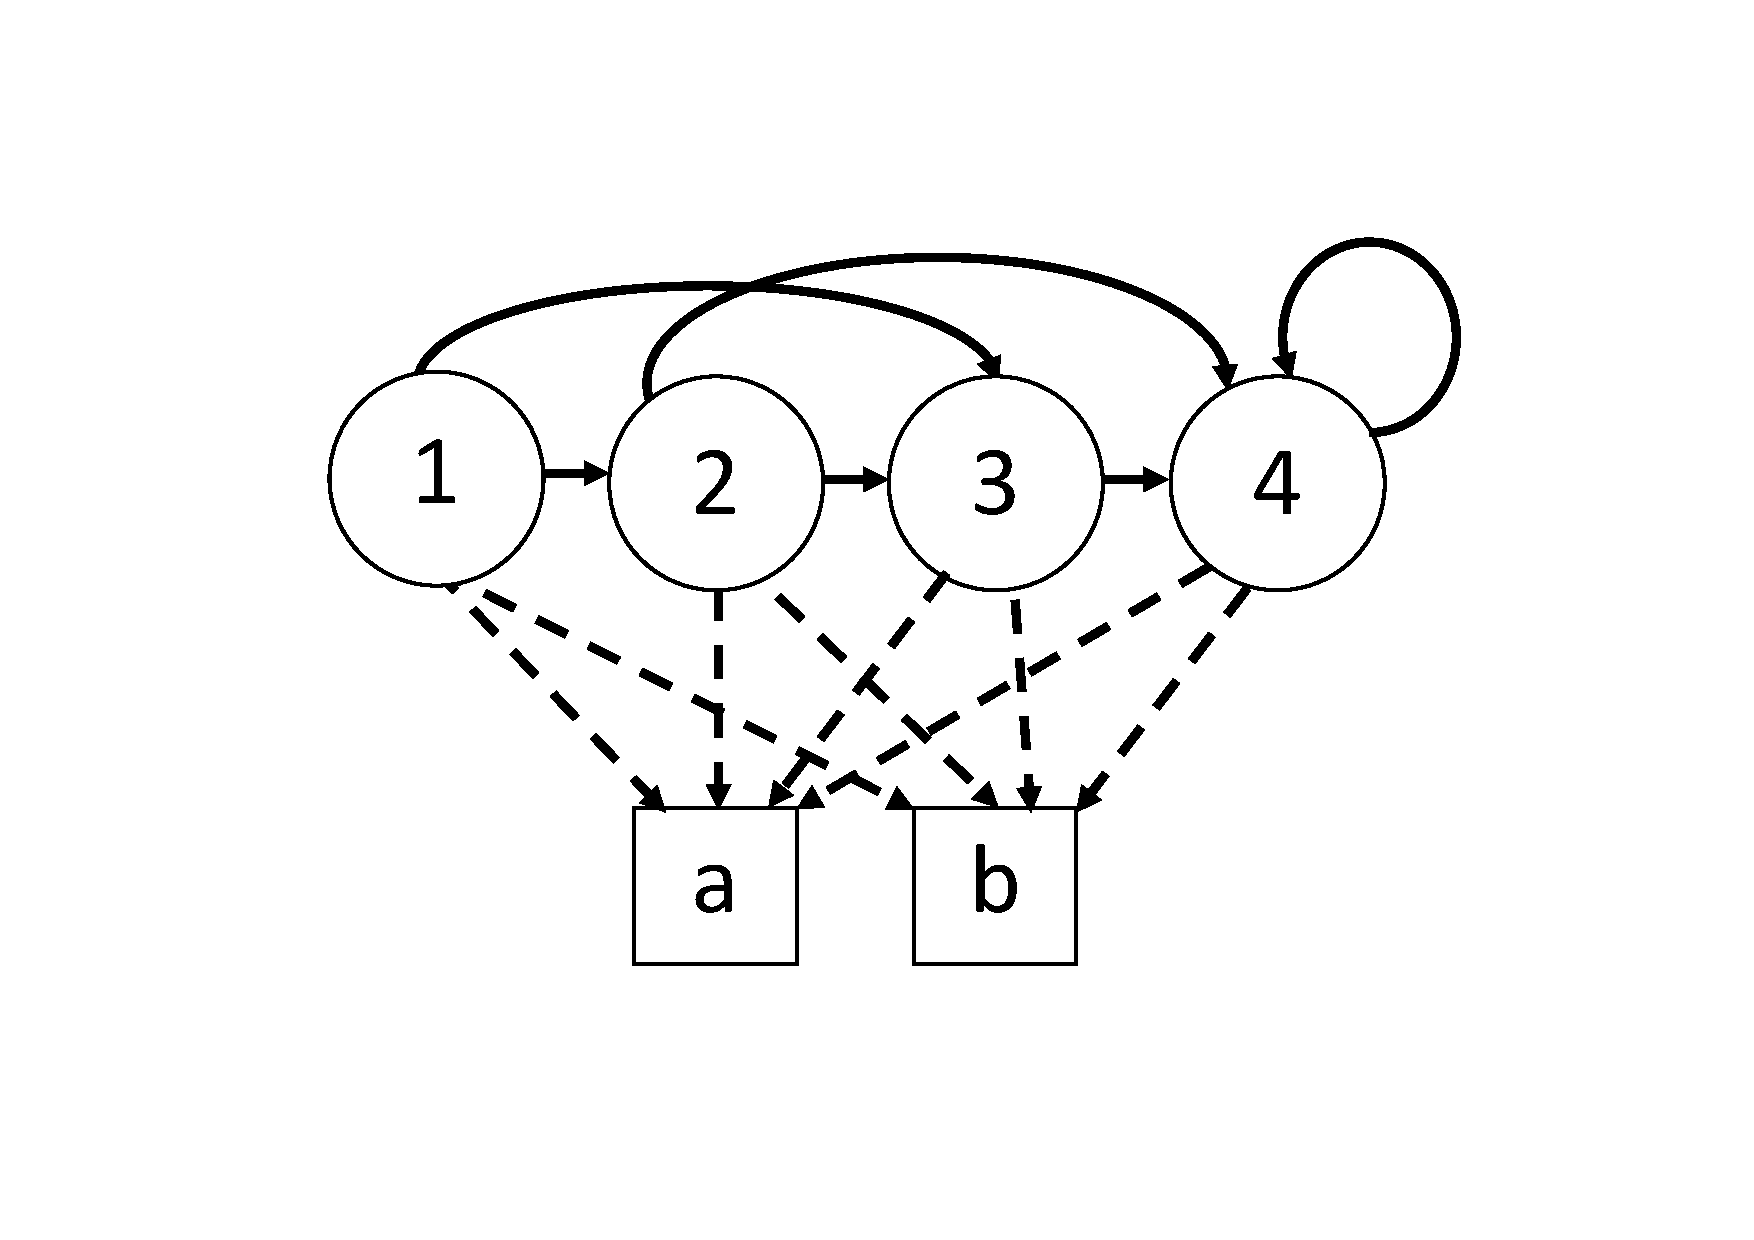
\includegraphics[width=0.7\textwidth]{ThesisFigs/HMMExample}
  \caption{A Hidden Markov Model. The underlying Markov Chain contains 4 states (depicted as circles) which emit two possible observations (a or b).}\label{ref:hmmex}
\end{figure}


Note now that a hidden Markov Model is entirely determined by the transition matrix $A$, the emissions matrix $B$ and the initial distribution $\bm{\pi}$ (noting that the dimensions $N$ and $M$ are encoded in the dimensions of the matrices) hence for convenience we may denote a HMM by
\begin{equation*}
\lambda = (A,B, \bm{\pi})
\end{equation*}

Hidden Markov Models were first introduced by in a series of papers by L.E Baum and others in the late 1960s ~\citep{baum1966statistical,baum1970maximization} and have been since used to study handwriting recognition~\citep{bunke1995off}, speech recognition ~\citep{juang1991hidden, jelinek1998statistical}, natural language modelling~\citep{manning1999foundations, jurafsky2002speech} and biological processes ~\citep{krogh1994hidden, durbin1998biological, lio1998models}.
\\
\\
Given these defintions there exist three basic problems which form the basis of using HMMs as a tool for machine learning
\begin{enumerate}
\item Given an observation sequence $\bm{O} = O_1,O_2,\dots,O_T$ and a HMM $\lambda$, what is $\mathbb{P}(\bm{O}|\lambda)$ - the probability that the observation sequence $\bm{O}$ was produced by $\lambda$?
\item Given a HMM $\lambda$ and an observation sequence $\bm{O} = O_1,O_2,\dots,O_T $ what is the state sequence of the underlying Markov chain in $\lambda$ which is most likely to have generated $\bm{O}$?
\item Given an observation sequence $\bm{O}$, how to do we choose the parameters of $\lambda = (A,B,\bm{\pi})$ which best optimise $\mathbb{P}(\bm{O}|\lambda)$?
\end{enumerate}

In fact the problem of sign language gesture recognition can be seen as instance of problems 3 and 1. First we take for each gesture $g$ a set of training data which are recordings of the joints in 3D space. This training data forms a collection of observation sequences $\bm{O_1}, \dots, \bm{O_n}$ which are used in a solution to problem 3 to parameterise a hidden Markov Model $\lambda_g$ to model the gesture.

Then given a fresh observation sequence $\bm{O}$ we can use a solution to problem 1 to compute $\mathbb{P}[\bm{O} | \lambda_g]$ for each $g$. We can then take the gesture $g$ for which this probability is maximised and, provided the probability exceeds some threshold, conclude that the gesture $g$ corresponds to the observation sequence $\bm{O}$. 

\subsection{The Forward and Backward Variables}
Suppose we are given an observation sequence $\bm{O} = O_1,O_2,\dots,O_T$ and a HMM $\lambda$ and we wish to solve the evaluation problem (problem 1). ~\citet{rabiner1989tutorial} notes that a direct computation of $\mathbb{P}[\bm{O}|\lambda]$ will take time order $\mathcal{O}(2TN^T)$ which is infeasible even for moderate values of $N$ and $T$. Instead we use a dynamic programming approach, the forward algorithm, introduced in~\citet{baum1968growth} and ~\cite{baum1970maximization}.

Define the \emph{forward variables} $\alpha_t(i)$ for each $1\leq t \leq T$ and $1 \leq i \leq N$ by
\begin{equation*}
\alpha_t(i) = \mathbb{P}[O_1, \dots, O_t, q_t=S_i | \lambda]
\end{equation*}
Then note these can be inductively computed by the following procedure 
\begin{align*}
&\alpha_1(i) = \pi_ib_i(O_1)\\
&\alpha_{t+1}(j) = \left[ \sum_{i=1}^{N} \alpha_{t}(i)a_{ij} \right]b_j(O_{t+1}) &\text{ for $1\leq t \leq T-1$ and $1 \leq j \leq N$}
\end{align*}
Finally we have
\begin{align*}
\mathbb{P}[\bm{O} | \lambda] &= \sum_{i=1}^N \mathbb{P}[\bm{O}, q_T = S_i | \lambda] = \sum_{i=1}^N \alpha_T(i)
\end{align*}
The set of forward variables can be computed by dynamic programming in $\mathcal{O}(N^2T)$ time and hence we can compute $\mathbb{P}[\bm{O} | \lambda]$ in this time -  a significant improvement over direct computation. This algorithm is the \emph{forward algorithm} for evaluation in HMMs. 

Symmetrically to the forward variables we can define a collection of \emph{backward variables} by
\begin{equation*}
\beta_t(i) = \mathbf{P}[O_{t+1}, O_{t+2}, \dots, O_T | q_t = S_i, \lambda]
\end{equation*}
Which gives the probability of a partial observation sequence from a time $t$ given the state of the HMM $\lambda$ at time t. These too can be computed iteratively as
\begin{align*}
&\beta_T(i) = 1 &\text{ for each } 1 \leq i \leq N \\
&\beta_t(i)  = \sum_{j=1}^N a_{i,j}b_j(O_{t+1})\beta_{t+1}(j) &\text{ for } t = T-1, T-2,\dots,1 \text{ and } 1 \leq i \leq N \\
\end{align*}
and these too can be computed by dynamic programming in $\mathcal{O}(N^2T)$ time. The backward variables are not needed in the solution to the evalutation problem but are used in the following section to re-parameterise hidden Markov Models. 

\subsection{Forward-Backward Algorithm}
The problem of parameterising a hidden Markov Model $\lambda$ is considerably more difficult than the other two problems of HMMs. In fact it is known that there is no analytic solution which provides a model $\lambda$ to maximise the probability of some observation sequence $\bm{O}$. Instead we must use local optimisation methods which given an initial parameterisation $\lambda_0$ iteratively improve it until $\mathbb{P}[\bm{O} | \lambda]$ reaches a local maximum. 

We will use a modified version of the \emph{Baum-Welch algorithm} introduced by~\citet{baum1970maximization} called the \emph{forward-backward algorithm}~\citep{rabiner1989tutorial} which is reproduced below. This algorithm is an instance of an expectation-maximization algorithm~\cite{moon1996expectation} which is a general technique used to determine maximum likelihood estimators in a number of machine learning models~\cite{bishop2006pattern}. \\
\\
For $t \in \{1, \dots, T-1\}$ and $i,j \in \{1, \dots, N\}$ define
\begin{equation*}
\gamma_t(i,j) = \mathbb{P}[q_t = S_i, q_{t+1}=S_j| \bm{O}, \lambda]
\end{equation*}
such that $\gamma_t(i,j)$ is the probability of being in state $S_i$ at time $t$ and transitioning to $S_j$ at the next time step given the HMM $\lambda$ and the observation sequence $\bm{O}$. The by definiton of the foward and backward variables we have
\begin{align*}
\gamma_t(i,j) &= \frac{\alpha_t(i)a_{ij}b_j(O_{t+1})\beta(j)}{\mathbb{P}[\bm{O}|\lambda]}	
\end{align*}
We can define for each $1 \leq t \leq T-1$ and each $1 \leq i \leq N$ the probability of being in state $i$ at time $t$ by
\begin{equation*}
\gamma_t(i) = \mathbb{P}[q_t = S_n | \bm{O}, \lambda] = \frac{\alpha_t(i)\beta_t(i)}{\mathbb{P}[\bm{O}|\lambda]}
\end{equation*}
and then we have
\begin{equation*}
\gamma_t(i) = \sum_{j=1}^N \gamma_t(i,j)
\end{equation*}
Now using these equations we can compute
\begin{align*}
&\sum_{t=1}^{T-1} \gamma_t(i) = \text{The expected number of transitions from $S_i$} \\
&\sum_{t=1}^{T-1} \gamma_t(i,j) =  \text{The expected number of transitions from $S_i$ to $S_j$}\\
\end{align*}
which can be used to reparameterise the model $\lambda = (A,B,\bm{\pi})$ as follows, set
\begin{align*}
\overline{\pi} &= \text{the expected number of times in state $S_i$ at time $1$} = \gamma_1(i) \\
\overline{a_{ij}} &= \frac{\text{the expected number if transitions from $S_i$ to $S_j$}}{\text{expected number of transitions from state $S_i$}} \\ 
				&= \frac{\sum_{t=1}^{T-1} \gamma_t(i,j)}{\sum_{t=1}^{T-1} \gamma_t(i)} \\
\overline{b}_j(k) &= \frac{\text{the expected number of times in state $S_j$ observing symbol $v_k$}}{\text{the expected number of times in state $S_j$}} \\
				&=\frac{\sum_{\stackrel{t=1}{O_t=v_k}}^{T}\gamma_t(j)}{\sum_{t=1}^T \gamma_t(j)}
\end{align*}
Then if denote $\overline{\lambda} = (\overline{A},\overline{B},\overline{\bm{\pi}})$ then it has been proven ~\citep{levinson1983introduction, baum1968growth} that either
\begin{enumerate}
\item $\mathbb{P}[\bm{O}|\overline{\lambda}] > \mathbb{P}[\bm{O}|\lambda]$ or
\item $\lambda$ is locally maximized with respect to $\mathbb{P}[\bm{O}|\lambda]$ and $\overline{\lambda} = \lambda$
\end{enumerate}
It follows that given an initial HMM $\lambda$ we may improve it to a locally optimal model for some observation sequence $\bm{O}$ via the following local search:
\begin{enumerate}
\item Whilst $\mathbb{P}[\bm{O}|\lambda]$ increases:
	\begin{enumerate}
		\item[i.] Compute the $\alpha_t(i)$, $\beta_t(i)$, $\gamma_t(i,j)$ and $\gamma_t(i)$
		\item[ii.] Compute the new parameters $\overline{A} = [\overline{a}_{ij}]$, $\overline{B} = [\overline{b}_j(k)]$ and $\overline{\bm{\pi}} = [\overline{\pi_1}, \dots, \overline{\pi_N}]$
		\item[iii.] Set $\lambda := \overline{\lambda}$
	\end{enumerate}
\item return $\lambda$
\end{enumerate}
Note that this algorithm may not actually terminate. In practice we threshold the increase of $\mathbb{P}[\bm{O}|\lambda]$ to ensure termination in a reasonable time. Further, in practice we will not have single observation sequence but rather a collection, perhaps from a variety of signers of different heights, genders, ages or dialects. In the implementation of our HMM framework we will modify this algorithm to work for multiple observation sequences. This will again increase the time complexity of the algorithm, however this problem is not so significant as in practice we will use this algorithm once per sign and save the parameterisations.

\subsection{Limitations of HMMs}
A significant limitation of hidden Markov Models is that they can have only a finite set $V$ of possible observations. In practice this can prevent us using a HMM to model a specific gesture exactly. Take for example the problem of detecting the gesture of a circle drawn on a 2D plane. We might create a hidden Markov Model in which the states of the Markov chain represent some specific points on the plane and want our matrix $B$ to be such that
\begin{align*}
&b_j(\bm{p}) = \mathbb{P}[\text{the pen is at point $\bm{p}$ at time $t$ } | q_t = S_j] &\text{ for each point $\bm{p}\in\mathbb{R}^2$}
\end{align*}
However as the plane is continuous and $V$ is finite this is not possible. One solution is the discretise the plane and have only a finite (but large) set of observation symbols. This method has been used with some success to distuingish between gestures with large variations, for example different tennis strokes~\citep{yamato1992recognizing}. However without sufficiently fine grained discretisation, which will severely impact the efficiency of our algorithms, our observation sequences will suffer from signal degradation. As we plan to model signed languages, in which certain subtle changes to a gesture can change the meaning {\color{green}[GIVEN AN EXAMPLE]}, it is likely signal degradation will impact on the accuracy of our system.

\section{Continuous Distribution HMMs}
Another solution to this problem is to use a \emph{continuous hidden Markov Model}~\citep{rabiner1989tutorial, dym2011hmm} which is defined similarly to a regular HMM except we allow an infinite number of observations symbols $O$ and define for each state $S_j$ the probability $b_j(O)$ to be drawn from a continuous finite mixture of distributions. That is
\begin{equation*}
b_j(O) = \sum_{m=1}^M c_{jm}f_m(O)
\end{equation*}
where $f_m$ are some (possibly parameterised) probability distribution functions and the $c_{jm}$ are mixture coefficients satisfying $\sum_m c_{jm} = 1$ for each $1 \leq j \leq N$. 

It has been shown that if the $f_m$ are log-concave functions then there exists a re-estimation tecnique for the continuous HMM which extends the forward-backward algorithm.~\cite{liporace1982maximum, juang1985maximum, juang1986maximum}. 

For the purposes of this project we will restrict ourselves to mixtures of Gaussian distributions as these the most commonly studied log-concave distributions. Then our $b_j(O)$ will take the form
\begin{equation*}
b_j(O) = \sum_{m=1}^M c_{jm}\mathcal{N}(O | \mu_{jm}, \Sigma_{jm})
\end{equation*}
where $\mu_{jm}$ is the mean vector and $\Sigma_{jm}$ the covariance matrix of the $m^\text{th}$ distribution in the mixture for state $S_j$, and  
\begin{equation*}
\mathcal{N}(O|\mu,\Sigma) = \frac{1}{(2\pi)^{d/2}\sqrt{|\Sigma|}}e^{\left(-\frac{1}{2}(x-\mu)^T\Sigma^{-1}(x-\mu)\right)}
\end{equation*}
with $d$ being the dimension of the observation $O$ (and hence of $\mu$ and $\Sigma$)~\citep{bishop2006pattern}.
\subsection{Re-estimation In Continuous HMMs}
Following the work of ~\citet{liporace1982maximum}, ~\citet{juang1985maximum} and~\citet{ juang1986maximum} we can extend the forward-backward algorithm to re-estimate the parameters of a continuous hidden Markov Model. The definition of the $\alpha_t(i)$, the $\beta_t(i)$ and the $\gamma_t(i)$ remain as before as doe the re-estimation of the stochastic matrix $A$ and initial state distribution $\bm{\pi}$. However we no longer have a matrix $B$ and instead must re-estimate the mixture coefficients $c_{jm}$, mean vectors $\mu_{jk}$ and covariance matrices $\Sigma_{jk}$. To do this we define
\begin{equation*}
\zeta_t(j,k) = \left[ \frac{\alpha_t(j)\beta_t(j)}{\sum_{j=1}^N \alpha_t(j)\beta_t(j)} \right]\left[ \frac{c_{jk}\mathcal{N}(O_t, \mu_{jk}, \Sigma_{jk})}{\sum_{m=1}^M c_{jm}\mathcal{N}(O_t, \mu_{jm},\Sigma_{jm})} \right]
\end{equation*}
and then compute
\begin{align*}
&\overline{c}_{jk} = \frac{\sum_{t=1}^T \zeta_t(j,k)}{\sum_{t=1}^T \sum_{m=1}^M \zeta_t(j,m)} 
&\overline{\mu}_{jk} = \frac{\sum_{t=1}^T \zeta_y(j,k)O_t}{\sum_{t=1}^T \zeta_t(j,k)} \\
\end{align*}
\begin{equation*}
\overline{\Sigma}_{jk} = \frac{\left(\sum_{t=1}^T \zeta_t(j,k)\right)(O_t - \mu_{jk})\otimes(O_t - \mu_{jk})}{\sum_{t=1}^T \zeta_t(j,k)}
\end{equation*}
for each $1 \leq j \leq N$ and $1 \leq k \leq M$. (Where $\otimes$ denotes the dyadic tensor product).
If we form a new continuous HMM $\overline{\lambda}$ with these new parameters then 
\begin{equation*}
\mathbb{P}[\bm{O}|\overline{\lambda}] \geq \mathbb{P}[\bm{O}|\lambda] 
\end{equation*}
and hence we may find a locally optimal model for some observation sequence $\bm{O}$ by a similar local search algorithm as for discrete HMMs.

\section{Previous Work}
Motivated by the success of hidden Markov Models for speech in the mid 1970s \citep{baker1975dragon, jelinek1975design} these models were adopted for gesture detection. ~\citet{yamato1992recognizing} used discrete HMMs with observations from a 2D camera to detect tennis strokes and later ~\citet{starner1995real} implemented a system to recognise American Sign Language in real-time using by continuous density hidden Markov Models. This system relied on a single camera and required the user to wear a pair of special gloves. By imposing a restricted grammar to only allow sentences of a particular structure they were able to achieve an accuracy of 97.0\% on an independent training set. 

More recently the SignSpeak project~\citep{dreuw2010signspeak}, which aims to use a 2D video camera and an extension of HMM techniques ~\citep{dreuw2009smoothed}, has received EU funding. This project aims to solve the problems of image extraction, sign recognition and language translation to provide a complete video-to-text system for sign language translation.

% ------------------------------------------------------------------------


%%% Local Variables: 
%%% mode: latex
%%% TeX-master: "../thesis"
%%% End: 

\chapter{Building a Hidden Markov Model for Isolated Signs}
\ifpdf
    \graphicspath{{Chapter2/Chapter2Figs/PNG/}{Chapter2/Chapter2Figs/PDF/}{Chapter2/Chapter2Figs/}}
\else
    \graphicspath{{Chapter2/Chapter2Figs/EPS/}{Chapter2/Chapter2Figs/}}
\fi
% ------------------------------------------------------------------------

\section{Scaling}
In the previous section we introduced methods for solving the evaluation and re-estimation problems for hidden markov models. These methods, whilst mathematically sound, introduce certain problems during implementation. In particular these solutions involve the products of a large number of probabilities, especially for long observation sequence. As a consequence when implemented these methods can cause errors due to underflow. To solve this problem we instead scale the intermediate $\alpha$, $\beta$ and $\gamma$ variables to prevent underflow in the intermediate calculations and choose to compute the logarithm of the probability in the evaluation problem. To do this we normalize the $\alpha_t(i)$ by setting
\begin{align*}
\overline{\alpha}_0(i) = \alpha_0(i) \text{ for each $0\leq i<N$} 
\end{align*}
and inductively defining for each $0\leq t < T$
\begin{align*}
c_t &= \frac{1}{\sum_{i=0}^{N-1}\overline{\alpha}_t(i)}\\
\hat{\alpha}_t(i) &= c_t\overline{\alpha}_t(i)\text{ for each $i$}\\
\overline{\alpha}_{t+1}(i) &= \sum_{i=0}^{N-1}\hat{\alpha}_t(i)a_{ij}b_j(O_{t+1}) \text{ for each $i$}\\
\end{align*}
We then have
\begin{align*}
1 = \sum_{i=0}^{N}\hat{\alpha}_{T-1}(i) &= c_0c_1\dots c_{T-1}\sum_{i=0}^{N}\alpha_{T-i}(j)\\
&=c_0c_1\dots c_{T-1}\mathbb{P}(\mathbf{O}|\lambda)\\
\end{align*}
and hence we can compute the log-probability of an observation sequence $\mathbf{O}$ by
\begin{equation*}
\log(\mathbb{P}[\mathbf{O}|\lambda]) = -\sum_{t=0}^{T-1}\log(c_t)
\end{equation*}
which allows us to determine probabilities which otherwise would be lost due to underflow. 

Further we can use the same scale factors on the $\beta$ variables as by inductively defining
\begin{align*}
\overline{\beta}_{T-1}(i) &= \beta_{T-1}(i) \\
\hat{\beta}_{t}(i) &= c_t\overline{\beta}_t(i)\\
\overline{\beta}_{t+1}(i) &= \sum_{j=0}^{N-1}a_{ij}b_j(\mathbf{O}_{t+1})\hat{\beta}_{t+1}(i)
\end{align*}
and redefining the $\gamma$ variables as
\begin{align*}
\gamma_t(i,j)&=\hat{\alpha}(i)a_{ij}b_j(\mathbf{O}_{t+1})\beta_{t+1}(j)\\
\gamma_t(i) &= \hat{\alpha}_t(i)\hat{\beta}_t(i)\frac{1}{c_t}
\end{align*}
It has been shown that using these variables in the re-estimation process still ensures that the the probability $\mathbb{P}[\mathbf{O}|\lambda]$ increases with each iteration. 

Using these methods we implemented a general purpose discrete hidden markov model class which can be instantiated with any number with any number of states, observation symbols and probabilities and trained from a collection of observation sequences.
\section{Observation Vector Quantization}

In order to use discrete observation hidden markov models for the problem of gesture recognition we must restrict the continuous observation space to a discrete set of observation symbols. This set of symbols should not be too large (say no more than 30 symbols) to ensure that the problems of training and evaluation can be solved quickly enough for use in a real-time recognition system. Further, an increase in the number of symbols will cause a decrease in the evaluated probability of a given observation sequence being generated by some HMM. If the symbol count is too high this can cause underflow in spite of the effects of scaling. Of course the symbol set should not be too small either as otherwise we might lose some subtle aspects of signs and cause similar signs to be indistinguishable.

To quantize our training data for a single sign we merged all of the points  into a single 3D point cloud and partitioned this point cloud into $k$ clusters. To do this we implemented Lloyd's algorithm to solve the k-means clustering problem. Then for any point we can assign an observation symbol in the range $\{1,\dots,k+1\}$ by taking the number of the cluster with the centroid closest (via Euclidean distance) to the point, or if the distance from the point to each of the means exceeds some threshold assigning the symbol $k+1$. 

\begin{figure}
        \centering
        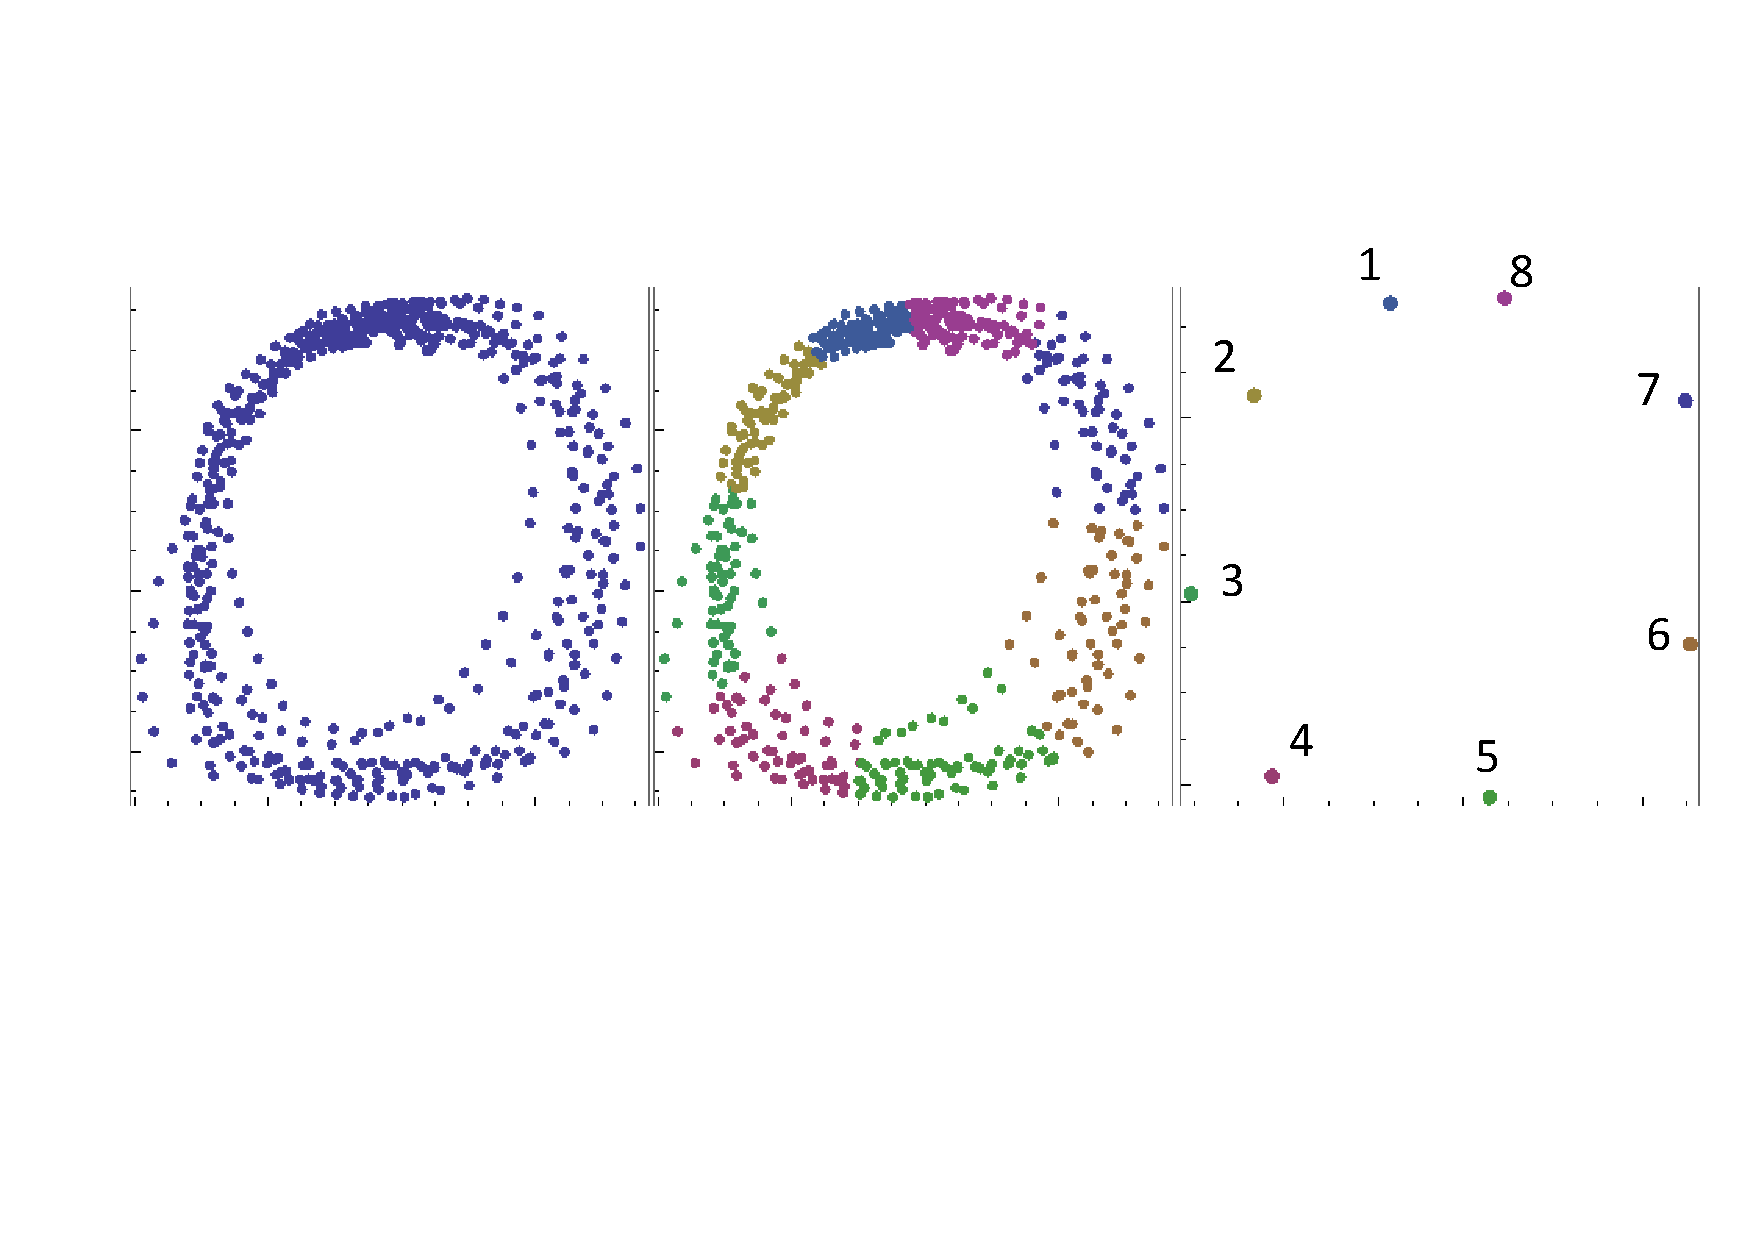
\includegraphics[width=0.9\textwidth]{ThesisFigs/ClusteringDiag}
        \caption{The K-Means method for vector quantization}\label{fig:kmeans}
\end{figure}

\section{Determining The Initial Topology and Parameters}
As our training method utilises a local search to improve our parameterisation its effectiveness will greatly depend on how we initialise our Hidden Markov Model. If the initial parameterisation is poor then even with a large training set we may fail to find a parameterisation which allows us to  recognise signs with high enough accuracy.

It has been shown that the topology of the underlying Markov Chain can greatly impact the effectiveness of a HMM for a given pattern recognition task~\citep{rabiner1989tutorial, jelinek1998statistical}. The two most common types of HMM (See figure ~\ref{fig:mctop}) are the \emph{ergodic model}, in which each state can transition to any other state in a finite number of steps and the \emph{left-right model} or Bakis model~\citep{bakis1976continuous} in which the state sequence is (non-strictly) increasing. The left-right model can be viewed as modelling a signal which changes through time, with each transition representing a movement forward in time. For that reason it is more suitable for modelling gestures or speech than other Markov Chain topologies and is the topology we choose for our Hidden Markov Models.

A left-right topology Markov chain is characterized by an upper triangular stochastic matrix $A$. We can further restrict our model to only allow jumps from a state $i$ to states $i \leq j \leq i+\Delta$ for some $\Delta$. This restriction can prevent the model being pushed, through re-parameterisation, into a trivial Markov chain which remains at the final state $N$ at all times. This can be seen as imposing a restriction on the velocity we can expect a signer's hand to move at - not allowing him to pass by too many states in quick succession.

As such we choose to intialize our HMMs as left-right models restricted to $\Delta = 1$ and initialise the stochastic matrix with form
\begin{equation*}
A =
 \begin{pmatrix}
  a_{11} & a_{12} & 0 & \cdots & 0 \\
  0 & a_{22} & a_{23} &\cdots & 0 \\
  \vdots  & \vdots  & \vdots & \ddots & \vdots  \\
  0 & 0 & \cdots & a_{(n-1)(n-1)}& a_{(n-1)n} \\
  0 & 0 & \cdots & 0& 1
 \end{pmatrix}
\end{equation*}
and define $\pi = [1,0, \dots, 0]$. Clearly if we initialise the non-zero $a_{ij}$ of A deterministically then we restrict ourselves to single outcome from the re-estimation procedure regardless of how many times we retry it, as such we choose to introduce some stochasticity by setting
\begin{align*}
&a_{ii} = 0.5 - r &a_{i(i+1)} = 0.5 + r
\end{align*}
 for some $r$ chosen uniformly from the interval $[-0.3, +0.3]$. This interval is chosen to ensure that none of the links are set too weakly and the forward transitions broken during re-estimation.

As we expect the system to differentiate a large number of signs it would be a major task to taylor the initialistions of each Hidden Markov Model to the sign it is expected to recognise. Hence, we choose to use the same initial estimation procedure for each HMM and do not make any inferences about the structure of the emissions matrix $B$ given the sign it is expected model. We initialise $B$ almost uniformly with
\begin{align*}
&b_{ij} = 1/M + r_{ij} &\text{for each $1\leq i \leq N$ and $1 \leq j \leq M$}
\end{align*}
where each $r_{ij}$ is some small random number and subject to the condition that the matrix $B$ remains stochastic.

The benefit of introducing stochasticity into the initial parameter estimations is that if the re-estimation procedure does not produce a sufficiently good parameterisation we can re-initialise our HMM and try again. That is to say we may use the forward-backward algorithm as part of a random restart hill climbing algorithm~\citep{russell1995artificial} to increase the chances that we will find a good parameterisation for the model.

\begin{figure}
        \centering
        \begin{subfigure}[b]{0.5\textwidth}
                \centering
                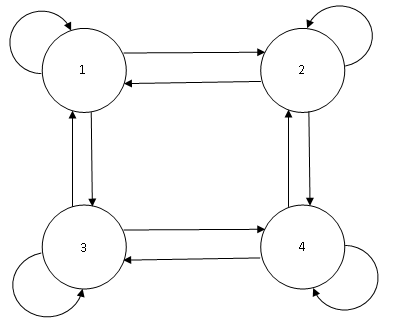
\includegraphics[width=1.0\textwidth]{ThesisFigs/erdogicMC}
                \caption{An Ergodic Markov Chain}
                \label{fig:unclust}
        \end{subfigure} 
        \begin{subfigure}[b]{0.5\textwidth}
                \centering
                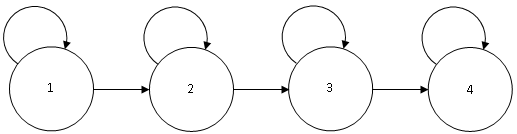
\includegraphics[width=1.0\textwidth]{ThesisFigs/del1LRMC}
                \caption{A $\Delta = 1$ Left-Right Markov Chain}
                \label{fig:clust}
        \end{subfigure}
	   \begin{subfigure}[b]{0.5\textwidth}
                \centering
                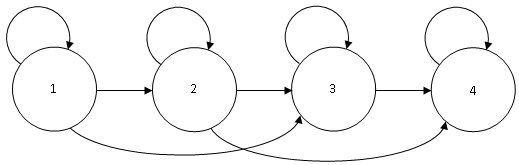
\includegraphics[width=1.0\textwidth]{ThesisFigs/del2LRMC}
                \caption{A $\Delta = 2$ Left-Right Markov Chain}
                \label{fig:clust}
        \end{subfigure}
        \caption{Different Markov Chain Topologies}\label{fig:mctop}
\end{figure}

\section{Predicting the Probability of a Sign}
Using the work of the previous sections we implemented a class \verb|DHMM| which can be instantiated to model a discrete observation Hidden Markov Model by providing initial parameters $A$, $B$ and $pi$ and also with a collection of less than $M$ vectors \verb|centroids[]| which specify how to translate observations from $\mathbb{R}^n$ (for any $n$) into discrete observations as described before. For convenience provided a means to save and load these parameters from file which means we need only go through the computationally expensive task of training the model once.

The Kinect Sensor provides a stream of real-time positions, as vectors in $\mathbb{R}^3$, of a number of joints in the body. A single \verb|DHMM| object can be trained on a collection of observations sequences of one of these joints, the left hand say, and be used to determine the probability that another observation sequence was produced by that HMM. If this probability is high enough we might conclude that this observations sequence matches the sign that produced the training data, however this procedure will only use observations from the left hand and ignore the information provided by the rest of the body.

One solution to this problem is to create an instance \verb|DHMM| which takes as its input streams vectors of $(\mathbb{R}^3)^J$ where $J$ is the number of joints we choose to track. This will allow us to train the model on full observations of the body and hence will take into account all of the information available through the Kinect Sensor in computing the probability that an observation sequence corresponds to a specific sign. This method introduces two problems however. The first is purely practical - the computations in the k-means clustering and training algorithms will become more and more expensive as the dimension of the observation vector grows and this will impact negatively on the perfomance of our sign recognition system.

The second issue is that this method ignores the prior knowledge we have about the joints of that body - that some are more dominant in the expression of a sign than others. For example, we know that the right hand is more dominant than the left and that both are more dominant than the elbows or shoulders. In fact the elbows and shoulders might be only worth considering when the hands alone cannot used to determine two different signs. As such we should not let the importance of each joint be determined algorithmically and should specify these parameters with care. For this we create $J$ seperate instances of \verb|DHMM|, each trained on a collection of observations sequences of a different joint. Then supposing we have trained a set of Hidden Markov Models $\Lambda = \{\lambda_1, \dots, \lambda_J\}$ for each joint, and observations sequences $\mathcal{O} = \{\mathbf{O}_1,\dots, \mathbf{O}_J\}$ which specify a stream for each joint over the course of one sign, we can compute the log-probability that this sequence corresponds to the sign used to train $\lambda_1, \dots, \lambda_J$ as a weighted sum
\begin{equation*}
\log(\mathbf{P}[\mathcal{O} | \Lambda ]) = \sum_{j=1}^{J} c_j \log(\mathbf{P}[\mathbf{O}_j | \lambda_j])
\end{equation*}
Where the weights $c_j$ are used to express the dominance of the $j^\text{th}$ joint in expressing a sign relative to the other joints.

We implemented the class \verb|SignModel| to correspond to this definition of $\Lambda$. This class contains a collection of \verb|DHMM| objects, with each corresponding to a joint of the skeleton provided by the Kinect Sensor as well as a set of weightings $c_1, \dots c_J$ along with a method to train the model by training the individual instances of \verb|DHMM| and a method which uses the above equation to compute the probability that a set of joint observation symbols corresponds to the sign used to train the model.

\subsection{Determining the Weightings}

\section{Building a Sign Classifier}

% ------------------------------------------------------------------------

%%% Local Variables: 
%%% mode: latex
%%% TeX-master: "../thesis"
%%% End: 

\chapter{My Third Chapter}
\ifpdf
    \graphicspath{{Chapter3/Chapter3Figs/PNG/}{Chapter3/Chapter3Figs/PDF/}{Chapter3/Chapter3Figs/}}
\else
    \graphicspath{{Chapter3/Chapter3Figs/EPS/}{Chapter3/Chapter3Figs/}}
\fi

\section{First Section of the Third Chapter}
\markboth{\MakeUppercase{\thechapter. My Third Chapter }}{\thechapter. My Third Chapter}
And now I begin my third chapter here ...

\subsection{first subsection in the First Section}
... and some more 

\subsection{second subsection in the First Section}
... and some more ...

\subsubsection{first subsub section in the second subsection}
... and some more in the first subsub section otherwise it all looks the same
doesn't it? well we can add some text to it ...

\subsection{third subsection in the First Section}
... and some more ...

\subsubsection{first subsub section in the third subsection}
... and some more in the first subsub section otherwise it all looks the same
doesn't it? well we can add some text to it and some more and some more and
some more and some more and some more and some more and some more ...

\subsubsection{second subsub section in the third subsection}
... and some more in the first subsub section otherwise it all looks the same
doesn't it? well we can add some text to it ...

\section{Second Section of the Third Chapter}
\markboth{\MakeUppercase{\thechapter. My Third Chapter }}{\thechapter. My Third Chapter}
and here I write more ...

% ------------------------------------------------------------------------


%%% Local Variables: 
%%% mode: latex
%%% TeX-master: "../thesis"
%%% End: 

\def\baselinestretch{1}
\chapter{Analysis and Conclusions}
\ifpdf
    \graphicspath{{Conclusions/ConclusionsFigs/PNG/}{Conclusions/ConclusionsFigs/PDF/}{Conclusions/ConclusionsFigs/}}
\else
    \graphicspath{{Conclusions/ConclusionsFigs/EPS/}{Conclusions/ConclusionsFigs/}}
\fi

\def\baselinestretch{1.66}


%%% ----------------------------------------------------------------------

% ------------------------------------------------------------------------

%%% Local Variables: 
%%% mode: latex
%%% TeX-master: "../thesis"
%%% End: 


\backmatter % book mode only
\appendix
\chapter{Appendix: Technical Details}

\section{Program Architecture}
This project was implemented in C\# using the Kinect SDK for Windows to provide access to the Kinect skeletal stream. The system was implemented using a Model-View-Controller architecure. The model here was the sign classifier which constitutes the majority of the project presented in this report whilst the controllers are the collection of classes we wrote to interface the Kinect sensor to the classifier. The view component consisted of a collection of simple user interfaces built using Windows Presentation Foundation to allow the user to record training, test and hold out data or to translate signs in real time by performing signs in front of the Kinect sensor.

Throughout the course of this project it became evident that there are a range of models we could have used in place of the discrete observation HMM. As such we used object oriented programming principles to ensure that the underlying workhorse statistical model which is used to build the \verb|signModel| class was easily interchangeable. For brevity we chose to forgoe the details of how interfaces were defined and used within the main report. Figure~\ref{fig:mvc} shows the full class hierarchy of the SignAlign system and how the Hidden Markov Model could be swapped for a different model easily.

\begin{figure}[t]
        \centering
        \includegraphics[width = 1.00\textwidth]{ThesisFigs/MVC}
        \caption{A UML diagram of the full SignAlign system}\label{fig:mvc}
\end{figure}

\section{Correctness Testing}
After implementing the \verb|DHMM|, \verb|signModel| and \verb|signClassifier| classes we verified their correctness by writing a collection of unit tests. However as we have built a statistical model the extent of our automated testing was limited to simple ``sanity checks'' and for this reason we omitted the details from the main report. We began by testing the likelihood evaluation and re-estimation procedure of the \verb|DHMM| class by comparing its results on a collection of predetermined test cases against those of the RHMM package written in R~\citep{RhmmPac}. Following this we went on to test the \verb|signModel| class by writing a collection of test re-estimations on a collection of observation sequences to ensure that the re-estimation procedure does indeed increase the likelihood of that \verb|signModel| generating those observation sequences. 

\section{Program Listing}
A full program listing for the SignAlign system is available at \\
\verb|https://github.com/Daniel-Nichol/sign-align|.
 
% ------------------------------------------------------------------------

%%% Local Variables: 
%%% mode: latex
%%% TeX-master: "../thesis"
%%% End: 

\chapter{Appdx B}

and here I put some more postamble ...

% ------------------------------------------------------------------------

%%% Local Variables: 
%%% mode: latex
%%% TeX-master: "../thesis"
%%% End: 


\bibliographystyle{plainnat}
%\bibliographystyle{Classes/CUEDbiblio}
%\bibliographystyle{Classes/jmb}
%\bibliographystyle{Classes/jmb} % bibliography style
\renewcommand{\bibname}{References} % changes default name Bibliography to References
\bibliography{References/references}{} % References file

\end{document}
